

\documentclass{beamer}
      \usepackage{lmodern}% http://ctan.org/pkg/lm
      \usepackage{float}
      \usepackage[english]{babel}
      \usepackage[utf8]{inputenc}
      \usepackage{amsmath}
      \usepackage{amssymb}
      \usepackage{color}
      \usepackage{subcaption}
      \usepackage{booktabs}
      \usepackage{tikz}
      \usepackage{multirow}
      \usetikzlibrary{decorations.pathreplacing}
      \usepackage{graphicx,epstopdf}
      \usepackage{cleveref}
      \usepackage{collcell} % loads array
      \usepackage{listings}
      \usepackage{algorithm}
      \usepackage{algpseudocode}
      \newcolumntype{m}{>{$} r <{$}}
      \newcolumntype{u}{>{$[\collectcell\si} l <{\endcollectcell]$}}
      \newcommand{\approxtext}[1]{\ensuremath{\stackrel{\text{#1}}{=}}}
      \newcommand{\matr}[1]{\mathbf{#1}}
      \newcommand{\partt}[2]{\ensuremath{\dfrac{\d {#1}}{\partial {#2}}}}
      \renewcommand{\d}[1]{\ensuremath{\operatorname{d}\!{#1}}} % non-italized differentials
      \newcommand{\h}[0]{\ensuremath{\hbar}} % hbar
      \def\changemargin#1#2{\list{}{\rightmargin#2\leftmargin#1}\item[]}
      \let\endchangemargin=\endlist 
      \usepackage{amsthm}
      \theoremstyle{plain}
      \newtheorem{thm}{theorem} % reset theorem numbering for each chapter
      \theoremstyle{definition}
      \newtheorem{defn}[thm]{definition} % definition numbers are dependent on theorem numbers
      \newtheorem{exmp}[thm]{example} % same for example numbers
      \bibliographystyle{natbib}
      \renewcommand{\theequation}{\thesection.\arabic{equation}}
      \newcommand{\ts}{\textsuperscript} 
      
      \definecolor{dkgreen}{rgb}{0,0.6,0}
      \definecolor{gray}{rgb}{0.5,0.5,0.5}
      \definecolor{mauve}{rgb}{0.58,0,0.82}

      \lstset{frame=tb,
        language=Java,
        aboveskip=3mm,
        belowskip=3mm,
        showstringspaces=false,
        columns=flexible,
        basicstyle={\small\ttfamily},
        numbers=none,
        numberstyle=\tiny\color{gray},
        keywordstyle=\color{blue},
        commentstyle=\color{dkgreen},
        stringstyle=\color{mauve},
        breaklines=true,
        breakatwhitespace=true,
        tabsize=3
      }


\begin{document}
\title{Hierarchical population systems}   
\author{Henrik Åhl} 
\date{\today} 

\frame{\titlepage} 
\section{} 
   \frame{
      \frametitle{Modeling population dynamics}
   }
   \frame{
      \frametitle{Modeling population dynamics}
      \begin{itemize}
            \item Three species: Foxes $\rightarrow$ rabbits $\rightarrow$ grass
      \end{itemize}
   }
   \frame{
      \frametitle{Modeling population dynamics}
      \begin{itemize}
            \item Three species: Foxes $\rightarrow$ rabbits $\rightarrow$ grass
            \item Three cases: Deterministic, stochastic, spatial
      \end{itemize}
   }
   \frame{
      \frametitle{Modeling population dynamics}
      \begin{itemize}
            \item Three species: Foxes $\rightarrow$ rabbits $\rightarrow$ grass
            \item Three cases: Deterministic, stochastic, spatial
            \item Parameters principally equivalent, although numerically
               different
      \end{itemize}
   }
   \frame{
      \frametitle{Equations}
      \centering
      \begin{align*}
         \frac{\partial F}{\partial t} &= \alpha_1 \frac{R(1-K_1F)}{1 + K_2R}F -
         \alpha_2 F \\
         \frac{\partial R}{\partial t} &= -\alpha_3 \frac{R(1-K_1F)}{1 + K_2R}F +
         \alpha_4 \frac{G(1-K_3R)}{1+ K_4G}R - \alpha_5R \\
         \frac{\partial G}{\partial t} &= -\alpha_6 \frac{G(1-K_3R)}{1 + K_4G}R +
         \alpha_7 (1-K_5G)G
      \end{align*}
   }
   \frame{
      \frametitle{Equations}
      \begin{align*}
         \frac{\partial F}{\partial t} &= \alpha_1 \frac{R(1-K_1F)}{1 + K_2R}F -
         \alpha_2 F \\
         \frac{\partial R}{\partial t} &= -\alpha_3 \frac{R(1-K_1F)}{1 + K_2R}F +
         \alpha_4 \frac{G(1-K_3R)}{1+ K_4G}R - \alpha_5R \\
         \frac{\partial G}{\partial t} &= -\alpha_6 \frac{G(1-K_3R)}{1 + K_4G}R +
         \alpha_7 (1-K_5G)G
      \end{align*}
      \begin{itemize}
         \item Theme: Logarithmic growth proportional to population size, limited derivatives
      \end{itemize}
   }
   \frame{
      \frametitle{Equations}
      \begin{align*}
         \frac{\partial F}{\partial t} &= \alpha_1 \frac{R(1-K_1F)}{1 + K_2R}F -
         \alpha_2 F \\
         \frac{\partial R}{\partial t} &= -\alpha_3 \frac{R(1-K_1F)}{1 + K_2R}F +
         \alpha_4 \frac{G(1-K_3R)}{1+ K_4G}R - \alpha_5R \\
         \frac{\partial G}{\partial t} &= -\alpha_6 \frac{G(1-K_3R)}{1 + K_4G}R +
         \alpha_7 (1-K_5G)G
      \end{align*}
      \begin{itemize}
         \item Theme: Logarithmic growth proportional to population size, limited derivatives
         \item Also diffusion of animals in spatial model
      \end{itemize}
   }

\section{Results}
   \frame{
      \frametitle{Results -- Deterministic}
      \begin{itemize}
         \item Oscillations and convergence
      \end{itemize}
      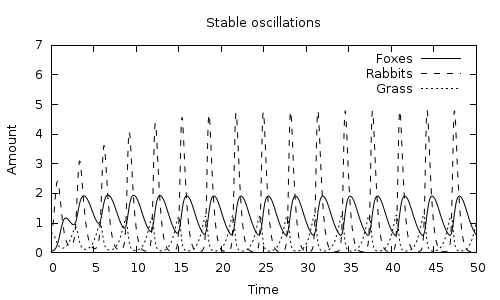
\includegraphics[width=.5\textwidth]{foxes_det_stable.png}%
      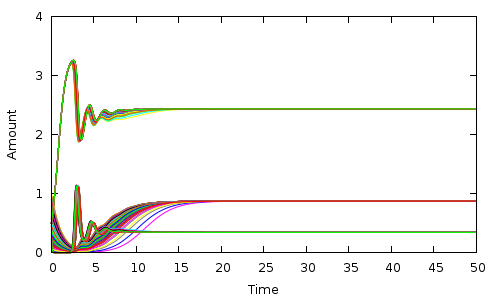
\includegraphics[width=.5\textwidth]{foxes_stable_all.png}
   }
\section{Results}
   \frame{
      \frametitle{Results -- Deterministic}
      \begin{itemize}
         \item Oscillations and convergence
      \end{itemize}
      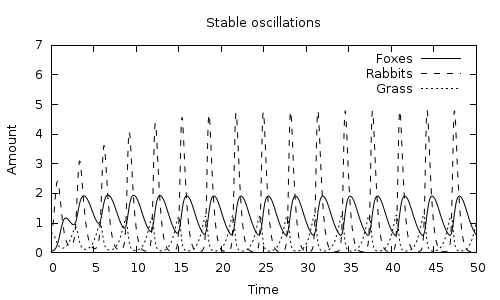
\includegraphics[width=.5\textwidth]{foxes_det_stable.png}%
      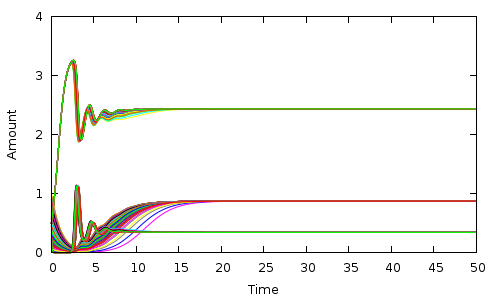
\includegraphics[width=.5\textwidth]{foxes_stable_all.png}
      \begin{itemize}
         \item Sanity check: Convergence abides to our equations
      \end{itemize}
   }
   \frame{
      \frametitle{Results -- Deterministic}
      \begin{itemize}
         \item Cyclic attractors (oscillations)
      \end{itemize}
      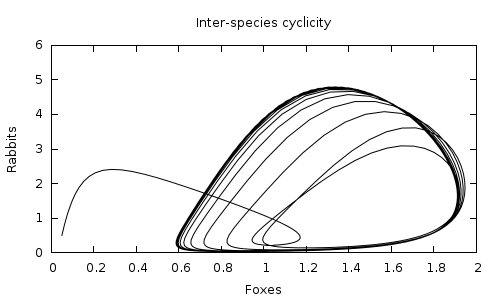
\includegraphics[width=.5\textwidth]{foxes_det_cyclicity_foxes_rabbits.png}%
      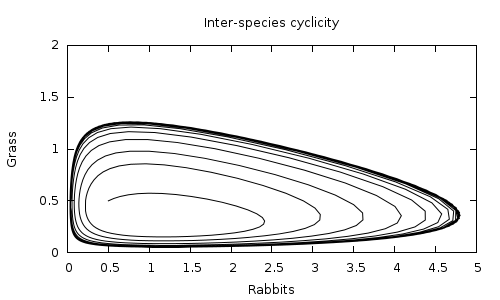
\includegraphics[width=.5\textwidth]{foxes_det_cyclicity_rabbits_grass.png}
   }
   \frame{
      \frametitle{Results -- Deterministic}
      \begin{itemize}
         \item Spiral attractors (convergence)
      \end{itemize}
      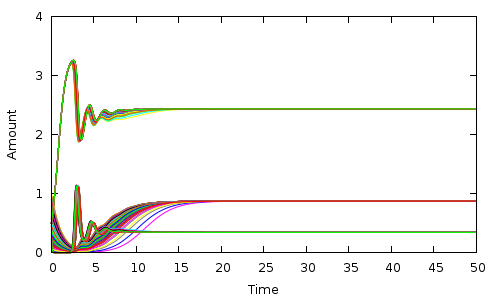
\includegraphics[width=.5\textwidth]{foxes_stable_all.png}%
      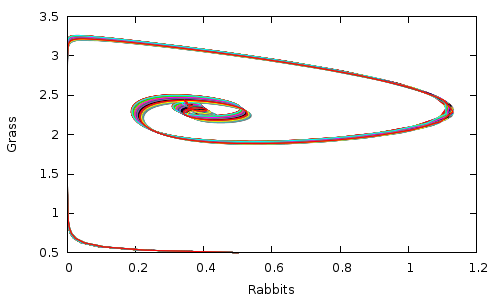
\includegraphics[width=.5\textwidth]{foxes_stable_rabbits_grass.png}
   }
   \frame{
      \frametitle{Results -- Stochastic}
      \begin{itemize}
         \item Possible to get oscillations
      \end{itemize}
   }
   \frame{
      \frametitle{Results -- Stochastic}
      \begin{itemize}
         \item Possible to get oscillations
         \item No stability (no attractors etc.)
      \end{itemize}
   }
   \frame{
      \frametitle{Results -- Stochastic}
      \begin{itemize}
         \item Possible to get oscillations
         \item No stability (no attractors etc.)
         \item Chance (risk) to exterminate species
      \end{itemize}
   }
   \frame{
      \frametitle{Results -- Stochastic}
      \begin{itemize}
         \item Possible to get oscillations
         \item No stability (no attractors etc.)
         \item Chance (risk) to exterminate species
      \end{itemize}
   }
   \frame{
      \frametitle{Results -- Stochastic}
      \begin{itemize}
         \item ``Stable'' oscillations
      \end{itemize}
      \centering
      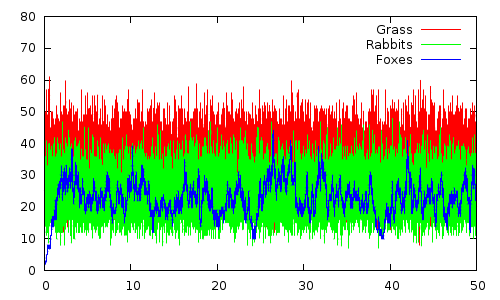
\includegraphics[width=.8\textwidth]{foxes_stochastic_oscillations.png}
   }
   \frame{
      \frametitle{Results -- Spatial}
      \begin{itemize}
         \item Stable oscillations and convergence
      \end{itemize}
      \centering
      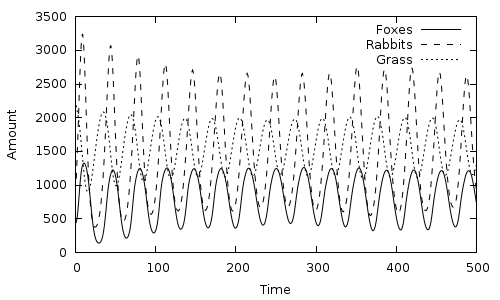
\includegraphics[width=.5\textwidth]{spatial_det_oscillations.png}
      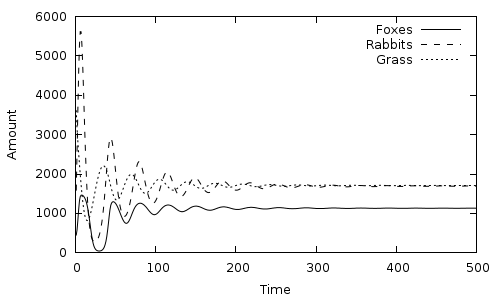
\includegraphics[width=.5\textwidth]{spatial_det_stable.png}
   }
   \frame{
      \frametitle{Results -- Spatial}
      \begin{itemize}
         \item Typical case: Foxes, rabbits, grass
      \end{itemize}
      \centering
      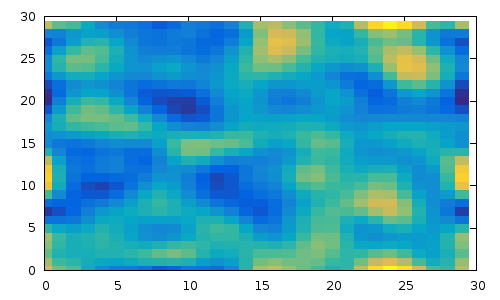
\includegraphics[width=.5\textwidth]{matrix_foxes.png}
      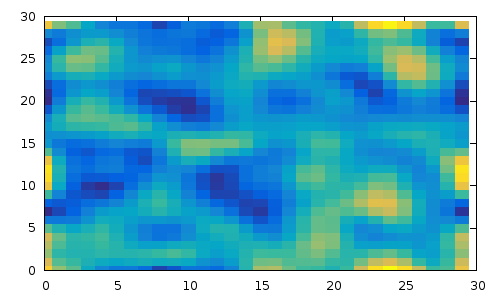
\includegraphics[width=.5\textwidth]{matrix_rabbit.png}\\
      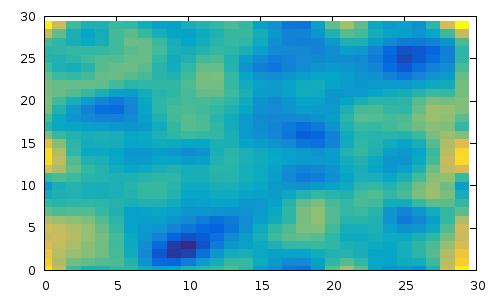
\includegraphics[width=.5\textwidth]{matrix_grass.png}
   }
   \frame{
      \frametitle{Results -- Spatial}
      \begin{itemize}
         \item Typical case: Foxes, rabbits, grass
      \end{itemize}
      \centering
      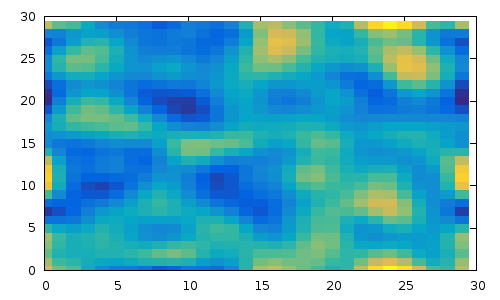
\includegraphics[width=.5\textwidth]{matrix_foxes.png}
      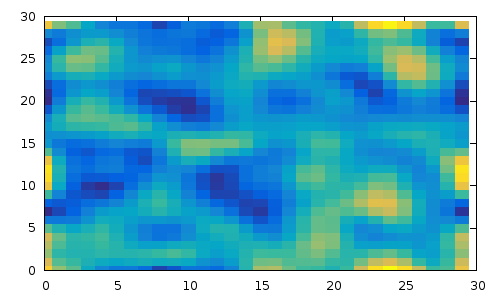
\includegraphics[width=.5\textwidth]{matrix_rabbit.png}\\
      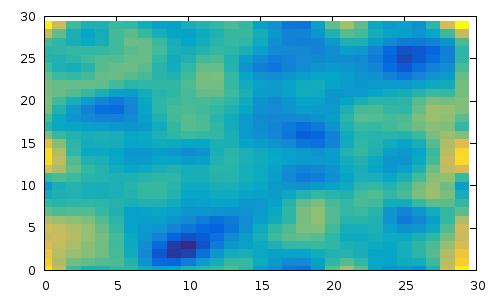
\includegraphics[width=.5\textwidth]{matrix_grass.png}
      \begin{itemize}
         \item Stabilization in value tends to mean stabilization in patterning
      \end{itemize}
   }
   \frame{
      \frametitle{Code}
      \begin{itemize}
         \item Implemented in Java
         \item Deterministic: RK-4
         \item Stochastic: Gillespie
         \item Spatial: Forward + Forward-Central Euler
      \end{itemize}
   }

\end{document}

